\documentclass[11pt,a4paper]{article}
\usepackage[T1]{fontenc}\usepackage[utf8]{inputenc}
\usepackage{lmodern,microtype,amsmath,amssymb,amsthm,mathtools}
\usepackage{booktabs,longtable,array,enumitem,xcolor,geometry,fancyhdr,hyperref,graphicx}
\geometry{margin=22mm}
\hypersetup{colorlinks=true,linkcolor=blue!55!black,urlcolor=blue,citecolor=blue!55!black,
 pdftitle={FIN ST1362--ST1451: Interval-Certified OA Optimization, Composite Identifiability and Sequential Inference},
 pdfauthor={Krzysztof Żuchowski}}
\pagestyle{fancy}\fancyhf{}\fancyhead[L]{FIN ST1362--ST1451}\fancyhead[R]{Release 10.99}\fancyfoot[C]{\thepage}\setlength{\headheight}{14pt}
\newtheorem{theorem}{Theorem}\newtheorem{proposition}[theorem]{Proposition}
\newcommand{\status}[1]{\textsf{[#1]}}

\begin{document}
\begin{titlepage}\centering\vspace*{14mm}
{\Huge\bfseries FIN ST1362--ST1451\par}\vspace{4mm}
{\LARGE Interval-Certified OA Optimization,\par}\vspace{2mm}
{\LARGE Composite Identifiability and Sequential Inference\par}\vspace{12mm}
{\Large Krzysztof \.Zuchowski\par}
{\normalsize Independent Researcher --- Fractal Information Theory Project\par}
{\normalsize ORCID: 0009-0002-0909-3613\par}\vspace{9mm}
{\large Six research rounds --- 90 programmes\par}
{\large Release 10.99 --- 31 August 2026\par}
\vfill
\begin{minipage}{.87\textwidth}\small
This report upgrades two strong numerical results from Release 10.98 to
outward interval certificates for a frozen decimal spectral model: the unique
return-gap maximizer and positive four-time separation from a declared
dephased-quantum nuisance box.  The result remains conditional on the frozen
Operational/State package and is not laboratory evidence.
\end{minipage}\vfill
{\small English mathematical and computational research report.}
\end{titlepage}

\begin{abstract}
ST1362--ST1451 strengthen the frozen Operational/State discrimination programme
of Release 10.98.  A decimal spectral model is declared exact, with seven
eigenvalues and multiplicities $(1,2,2,2,2,2,1)$.  Outward interval arithmetic
then proves that the absolute classical--quantum return gap on $[0,10]$ has one
global maximum.  Its time lies in
\[
[0.59453078,0.59453079]
\]
and its value lies in
\[
[0.4112409998076315,0.41124099980763185].
\]
The proof covers $[0,10]\setminus[0.59,0.60]$ with 4995 Taylor interval boxes,
proves positivity and strict concavity on the remaining interval, and brackets
the unique derivative zero.  This upgrades the previous dense-grid result to a
theorem for the frozen decimal spectrum, not for symbolic kernel parameters.

The four-time composite problem is also certified.  A complete cover of 1000
rectangles in
$(\alpha,\gamma)\in[0.9,1.1]\times[0,100]$ proves that no member of the
declared energy-dephased quantum family reproduces the classical return curve
at times $(0.3,0.6,1.2,2.0)$.  The residual sum of squares satisfies
\[
\mathrm{RSS}\ge0.046692011213846946,
\]
so at least one time has absolute residual at least $0.10804167160619894$.
A point candidate has RSS $0.05239469837327923$; its optimizer status is not
proved.

Preparation, detector and loss budgets are made explicit.  The full twelve-
vertex likelihood reduces without information loss to seven cyclic distance
classes.  Its Chernoff information is $0.13647980004881377$, versus
$0.10028599984500335$ for binary return.  A conservative Chernoff bound gives
29 full-record shots for equal-prior error below one percent in the two simple
hypotheses.  The interval composite certificate yields a much more
conservative 1146 binary shots per time by a Hoeffding union bound.

For the simple seven-class models, the likelihood ratio is an anytime-valid
e-process.  Symmetric boundaries $100$ and $0.01$ control either wrong
decision by one percent under optional stopping.  A naively refitted composite
likelihood is not automatically an e-process.  Protocol 10.99, its fail-closed
sequential validator and synthetic fixtures implement these distinctions.

No state ontology, dimensional clock value, apparatus, raw natural event,
independent custody or physical validation is supplied.  The certificates
make a conditional $OA$ mathematically sharper; they do not promote it into
strict FIN physics.
\end{abstract}

\tableofcontents\newpage

\section{Frozen decimal spectral model}

The interval theorems treat the following decimal inputs as exact:
\begin{align*}
\lambda={}&(0, 0.75412115420707981, 1.5770495144276093,\\
&1.9614068619764458, 2.1995688493332102,\\
&2.2986062720790965, 2.3421820411462999),
\end{align*}
with multiplicities $(1,2,2,2,2,2,1)$.  This freezes a reproducible finite
problem and removes binary floating ambiguity inside the certificate.

It does not certify an exact symbolic spectrum from $(\omega,\phi,\beta,\eta)$
or an interval matrix containing every reconstruction error.  That lift is a
recommended next problem.

Define
\[
C(t)=\frac1{12}\sum_km_ke^{-\lambda_kt},qquad
a(t)=\frac1{12}\sum_km_ke^{-i\lambda_kt},qquad
Q(t)=|a(t)|^2,
\]
and $F(t)=Q(t)-C(t)$.  The optimized quantity is $|F(t)|$.

\section{Round I: ST1362--ST1376 --- certified time optimum}

\subsection{Global cover}

The region
\[
[0,10]\setminus[0.59,0.60]
\]
is partitioned into 4995 intervals of width $0.002$.  For a box $I$ with
midpoint $m$ and radius $r=0.001$, the mean-value enclosure is
\[
 |F(I)|\le |F(m)|+r\sup_{t\in I}|F'(t)|,
\]
with every function evaluation outward-rounded by interval arithmetic.

At $t=0.5945308$ the certified lower value is
$0.4112409998076313$.  The largest upper bound outside the target interval is
$0.41123791023521883$, attained by the cover cell $[0.588,0.59]$.  The strict
exclusion margin is
\[
3.089572412462438\times10^{-6}>0.
\]

\subsection{Unique maximum inside the target interval}

On $[0.59,0.60]$, interval arithmetic gives
\[
F(t)\in[0.3966679604508919,0.425775515327064],
\]
so $|F|=F$, and
\[
F''(t)\in[-1.6864459900506021,-1.3685959622948138].
\]
Thus $F$ is strictly concave.  The endpoint derivative enclosures are
\[
F'(0.59453078)in
[2.5452303868190474,2.5452303868190486]\times10^{-9},
\]
\[
F'(0.59453079)=
-1.2746103229835985\times10^{-8}.
\]
The derivative has one and only one zero in the bracket.

\begin{theorem}[unique frozen-decimal return-gap maximum]
For the declared decimal spectrum, $|Q(t)-C(t)|$ has exactly one global
maximizer on $[0,10]$.  It lies in
$[0.59453078,0.59453079]$, and the maximum value lies in
\[
[0.4112409998076315,0.41124099980763185].
\]
\end{theorem}

This converts a previous strong numerical observation into an interval theorem
within the declared input scope.

\section{Round II: ST1377--ST1391 --- composite identifiability}

The nuisance family is the energy-dephased quantum return
\[
Q_{\alpha,\gamma}(t)=\frac1{12^2}\sum_{j,k}m_jm_k
e^{-\frac12\gamma(\lambda_j-\lambda_k)^2\alpha t}
\cos((\lambda_j-\lambda_k)\alpha t),
\]
with
\[
0.9\le\alpha\le1.1,qquad0\le\gamma\le100.
\]
The classical target is sampled at
$T=(0.3,0.6,1.2,2.0)$, and
\[
R(\alpha,\gamma)=\sum_{t\in T}
\bigl(Q_{\alpha,\gamma}(t)-C(t)\bigr)^2.
\]

The nuisance rectangle is covered by 20 clock cells of width $0.01$ and 50
dephasing cells of width $2$, for 1000 outward interval cells.  Summing the
lower bounds of the four squared residual intervals gives
\[
\boxed{R(\alpha,\gamma)\ge0.046692011213846946.}
\]
The weakest cover cell is
$\alpha\in[1.09,1.10]$, $\gamma\in[10,12]$; this need not contain the actual
optimizer.  The point $(1.1,12.373117825382856)$ gives
\[
R=0.05239469837327923.
\]

\begin{theorem}[four-time composite identifiability]
No quantum model in the declared $(\alpha,\gamma)$ box exactly reproduces the
four classical return probabilities.  At least one of the four absolute
residuals is at least
\[
\sqrt{0.046692011213846946/4}
=0.10804167160619894.
\]
\end{theorem}

This is not a theorem over all Lindblad dynamics.  The clock band and the
energy-dephasing family are paid premises.

\begin{figure}[ht]
\centering
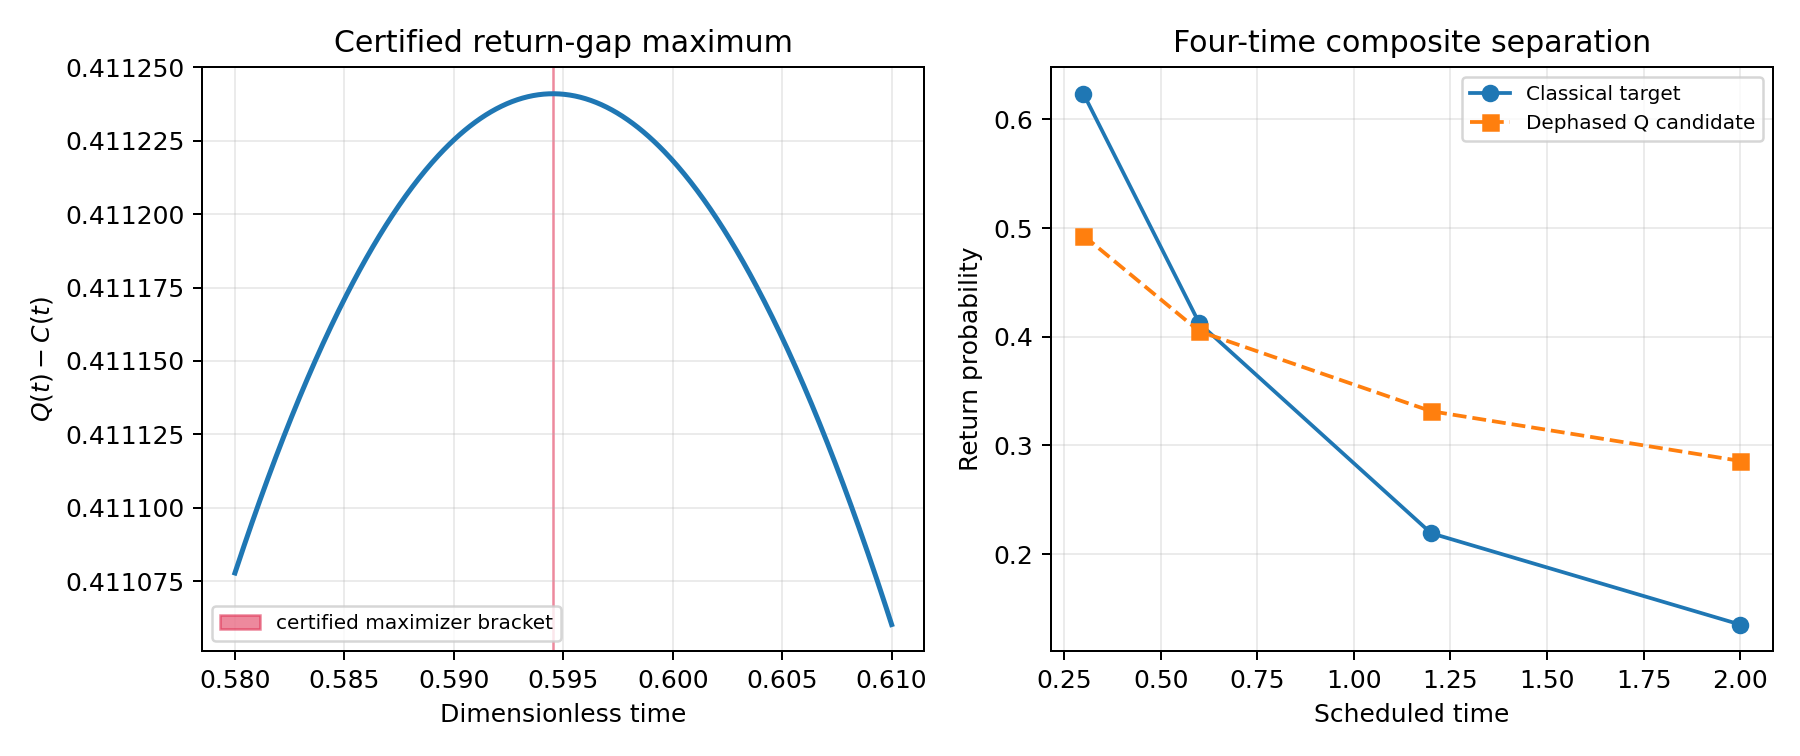
\includegraphics[width=.98\textwidth]{FIN_ST1362_ST1451_Figures/certified_oa_upgrade.png}
\caption{Left: the certified maximizer bracket (visually thinner than a pixel).
Right: the four-time classical target and one near-minimizing dephased quantum
candidate.}
\end{figure}

\section{Round III: ST1392--ST1406 --- calibration and errors}

At the practical time $t=0.6$, the ideal return gap is
\[
D=0.41121822546536.
\]

If both hypotheses suffer independent unknown scalar probability errors of at
most $\epsilon$, the triangle inequality gives
\[
D_{\rm observed}\ge D-2\epsilon.
\]
Thus binary-return identifiability is guaranteed for
$\epsilon<D/2\approx0.2056091$.  Assigning independent preparation and detector
budgets $0.05$ each yields the conservative combined bound
\[
D_{\rm observed}\ge D-2(0.05+0.05)=0.21121822546536>0.
\]

For common uniform source contamination,
\[
p'_H=(1-\epsilon)p_H+\epsilon/12,
\]
the gap scales exactly by $1-\epsilon$.  Ten percent contamination therefore
retains a gap about $0.3701$.

A binary confusion channel with false-positive rate $a$ and false-negative
rate $b$ maps
\[
p\mapsto a+(1-a-b)p,
\]
and scales a common calibrated gap by $|1-a-b|$.  The surface $a+b=1$ is
nonidentifying.

Known uniform loss preserves click-conditioned vertex probabilities but
changes the attempt-level click rate.  If no-clicks are discarded, unknown
loss is invisible.  Vertex-dependent efficiencies require a calibrated
confusion/efficiency matrix and are not covered by the scalar model.

\section{Round IV: ST1407--ST1421 --- full likelihood}

At $t=0.6$, the full event log-likelihood ratio is
\[
\ell(x)=\log\frac{q_x}{p_x},qquad
L_n=\sum_xn_x\ell(x).
\]
Reflection symmetry makes the cyclic distance $d=0,1,\ldots,6$ a sufficient
seven-class statistic: the vertices $+d$ and $-d$ have identical likelihood
ratios.  Thus the twelve labels compress to seven without information loss for
the frozen simple hypotheses.

The full directional divergences are
\[
D(C\|Q)=0.706146122009315,qquad
D(Q\|C)=0.4134894066196461.
\]
The optimized Chernoff information is
\[
\mathcal C_{\rm full}=0.13647980004881377,
\]
compared with
$\mathcal C_{\rm return}=0.10028599984500335$.  The gain ratio is about $1.36$.
The single-event total variation is $0.4112182254653598$, giving equal-prior
Bayes error $0.2943908872673201$.

The standard product Chernoff bound
\[
P_e(n)\le\frac12e^{-n\mathcal C}
\]
gives 29 full-record shots as a sufficient, not minimal, bound for error below
one percent.  The analogous binary Chernoff bound needs 40; direct exact
binomial tails from Release 10.98 happened to need only 29.

For the composite certificate, the fact that at least one time differs by
$\delta=0.1080416716$ gives a conservative Hoeffding/union design of 1146
binary shots per time, or 4584 total.  This is proof-safe but not optimized.

\section{Round V: ST1422--ST1436 --- anytime-valid inference}

For iid seven-class events define
\[
E_n=\prod_{i=1}^n\frac{q(X_i)}{p(X_i)}.
\]
Under the classical simple hypothesis, $(E_n)$ is a nonnegative mean-one
martingale.  Under the quantum simple hypothesis, $(1/E_n)$ is one.  Ville's
inequality therefore proves that the symmetric rule
\[
E_n\ge100\Rightarrow Q,qquad
E_n\le0.01\Rightarrow C
\]
has either wrong-boundary probability at most $0.01$, even under optional
stopping.

Expected log-likelihood growth is $0.4134894$ per event under $Q$ and
$-0.7061461$ under $C$.  Dividing $\log100$ by these rates gives rough Wald
scales of $11.14$ and $6.52$ events, respectively; overshoot makes these
approximations, not guarantees.

Optional inspection is safe only because the model and likelihood are frozen.
Maximizing a nuisance likelihood after each event does not automatically
produce an e-process.  A valid composite sequential test requires a
predeclared mixture, test martingale or another proved domination construction.

Protocol \path{FIN_ST1422_ST1436_Protocol_10_99.json} freezes the decimal
spectrum, seven-class probabilities, sequential boundaries, composite box,
certified RSS lower bound, calibration budgets and role separation.  The
fail-closed validator rejects invalid classes and malformed protocols.  Seeded
synthetic fixtures stop on the correct boundaries at 6 and 9 events; they are
code tests, not data.

\section{Round VI: ST1437--ST1451 --- final status}

\begin{longtable}{@{}p{.34\textwidth}p{.21\textwidth}p{.35\textwidth}@{}}
\toprule
Result & Status & Boundary \\
\midrule\endhead
unique return-gap maximizer & \status{Interval-proven} & frozen decimal spectrum, $[0,10]$ \\
four-time nuisance separation & \status{Interval-proven} & $\alpha\in[.9,1.1]$, energy dephasing $[0,100]$ \\
preparation/detector budgets & \status{Proven bounds} & scalar/common models \\
seven-class sufficient likelihood & \status{Proven} & frozen simple hypotheses \\
29-shot Chernoff sufficiency & \status{Proven bound} & full simple-record iid model \\
1146 shots/time composite design & \status{Proven conservative} & Hoeffding union bound \\
anytime-valid LR boundaries & \status{Proven} & simple hypotheses only \\
composite e-process & \status{Open} & naive plug-in invalid \\
protocol/validator & \status{Constructed/tested} & synthetic fixtures \\
laboratory realization & \status{Absent} & no apparatus/events/custody \\
\bottomrule
\end{longtable}

These results strengthen the conditional $OA$.  They do not derive $OA$ from
the strict kernel and do not choose a physical state ontology.

The protocol distinguishes mass-mixing dynamics from coherent unitary
dynamics inside the proposed total state.  It does not observe literal
annihilation or nonexistence of the whole nadsoliton.

\section{Recommended next programmes}

\begin{enumerate}
\item lift decimal certificates to interval uncertainty in the entries of $A$;
\item certify eigenvalue clusters from an interval matrix;
\item solve the minimax four-time likelihood allocation;
\item construct a valid mixture e-process over $(\alpha,\gamma)$;
\item add a calibrated preparation simplex;
\item add a detector confusion/efficiency polytope;
\item optimize time allocation rather than equal counts;
\item use seven-class sequential records in the composite test;
\item transport the protocol through the exact $12\to24$ refinement;
\item derive one platform-specific forward model without claiming realization;
\item freeze independent calibration and custody forms;
\item seek external review before any event collection.
\end{enumerate}

Stop after a spectrum outside the frozen model, nuisance outside the certified
box, unregistered detector law, postselection without no-clicks, adaptive
plug-in likelihood or post-unblinding protocol edit.

\section{Final conclusion}

\begin{quote}
The main numerical discoveries of Release 10.98 are now theorem-grade inside a
precisely frozen decimal model.  The optimal return time is unique, and a
calibrated four-time record cannot be exactly reproduced by the declared
dephased-quantum family.  Full spatial records and anytime-valid likelihood
ratios materially improve the simple-hypothesis test.  The remaining frontier
is no longer whether a separation exists, but whether it survives interval
uncertainty in the operator, a complete hardware nuisance model and independent
physical realization.
\end{quote}

\appendix
\section{Six-round ledger}
\begin{longtable}{@{}p{.18\textwidth}p{.33\textwidth}p{.39\textwidth}@{}}
\toprule
Range & Object & Verdict \\
\midrule\endhead
ST1362--ST1376 & interval time optimization & unique global maximum certified \\
ST1377--ST1391 & composite interval cover & positive RSS lower bound \\
ST1392--ST1406 & preparation/detector/loss & explicit calibration budgets \\
ST1407--ST1421 & full multinomial likelihood & seven sufficient classes and shot bounds \\
ST1422--ST1436 & sequential inference & simple-model e-process and protocol 10.99 \\
ST1437--ST1451 & synthesis & conditional theorem upgrade, evidence absent \\
\bottomrule
\end{longtable}

\section{Reproducibility}
The authoritative result sets run from
\path{FIN_ST1362_ST1376_Results.json} through
\path{FIN_ST1437_ST1451_Results.json}.  Each contains fifteen programmes and
packet SHA-256 references.  The combined test
\path{test_fin_st1362_st1451.py} verifies all ninety packets, interval margins,
composite lower bound, error budgets, likelihood gain, sequential protocol,
figure and nonpromotion gates.

\section{Nonclaims}
No symbolic-kernel interval theorem, complete open-quantum library, physical
clock calibration, state ontology, apparatus, raw event, independent custody,
legacy bridge, selector, Standard Model, gravity, $L_{\rm total}$ or Theory of
Everything is established.  All future FIN PDFs remain English.

\begin{thebibliography}{9}
\bibitem{moore} R. E. Moore, R. B. Kearfott and M. J. Cloud, \emph{Introduction to Interval Analysis}, SIAM.
\bibitem{cover} T. M. Cover and J. A. Thomas, \emph{Elements of Information Theory}, Wiley.
\bibitem{ville} J. Ville, \emph{Etude critique de la notion de collectif}, Gauthier-Villars.
\end{thebibliography}
\end{document}
